\clearpage
\chapter{Projektorganisation}
\section{Aufgabenverteilung}
Wie bereits in \ref{sec:herangehensweise} erläutert wurde, war das Projektteam sehr gut ausbalanciert und brachte ein breites Spektrum an technischen und wirtschaftlichen Verständnis mit. Um die konkrete Aufgabenteilung darzustellen, sind nachfolgende alle Aufgaben und deren Bearbeiter beschrieben. 
\begin{enumerate}
	\item Coding
	\begin{itemize}
		\item Miriam Wolf, Erik Schmidt, Ewald Anselm
	\end{itemize} 
	\item JUnit-Tests: Erstellung, Realisierung und Implementierung
	\begin{itemize}
		\item Rebekka Henn, Luisa Karl
	\end{itemize} 
	\item Coding Layout: Erstellung, Realisierung und Implementierung
	\begin{itemize}
		\item Ewald Anselm, Erik Schmidt
	\end{itemize} 
	\item Markt Algorithmen: Erstellung, Realisierung und Implementierung
	\begin{itemize}
		\item Tilman Heß
	\end{itemize} 	
	\item Dokumentation und Präsentation
	\begin{itemize}
	\item Nico Feil
	\end{itemize}
\end{enumerate}
\clearpage
\section{Meilensteine}\label{sec:meilenstein}
\begin{figure}[!h]
	\centering
	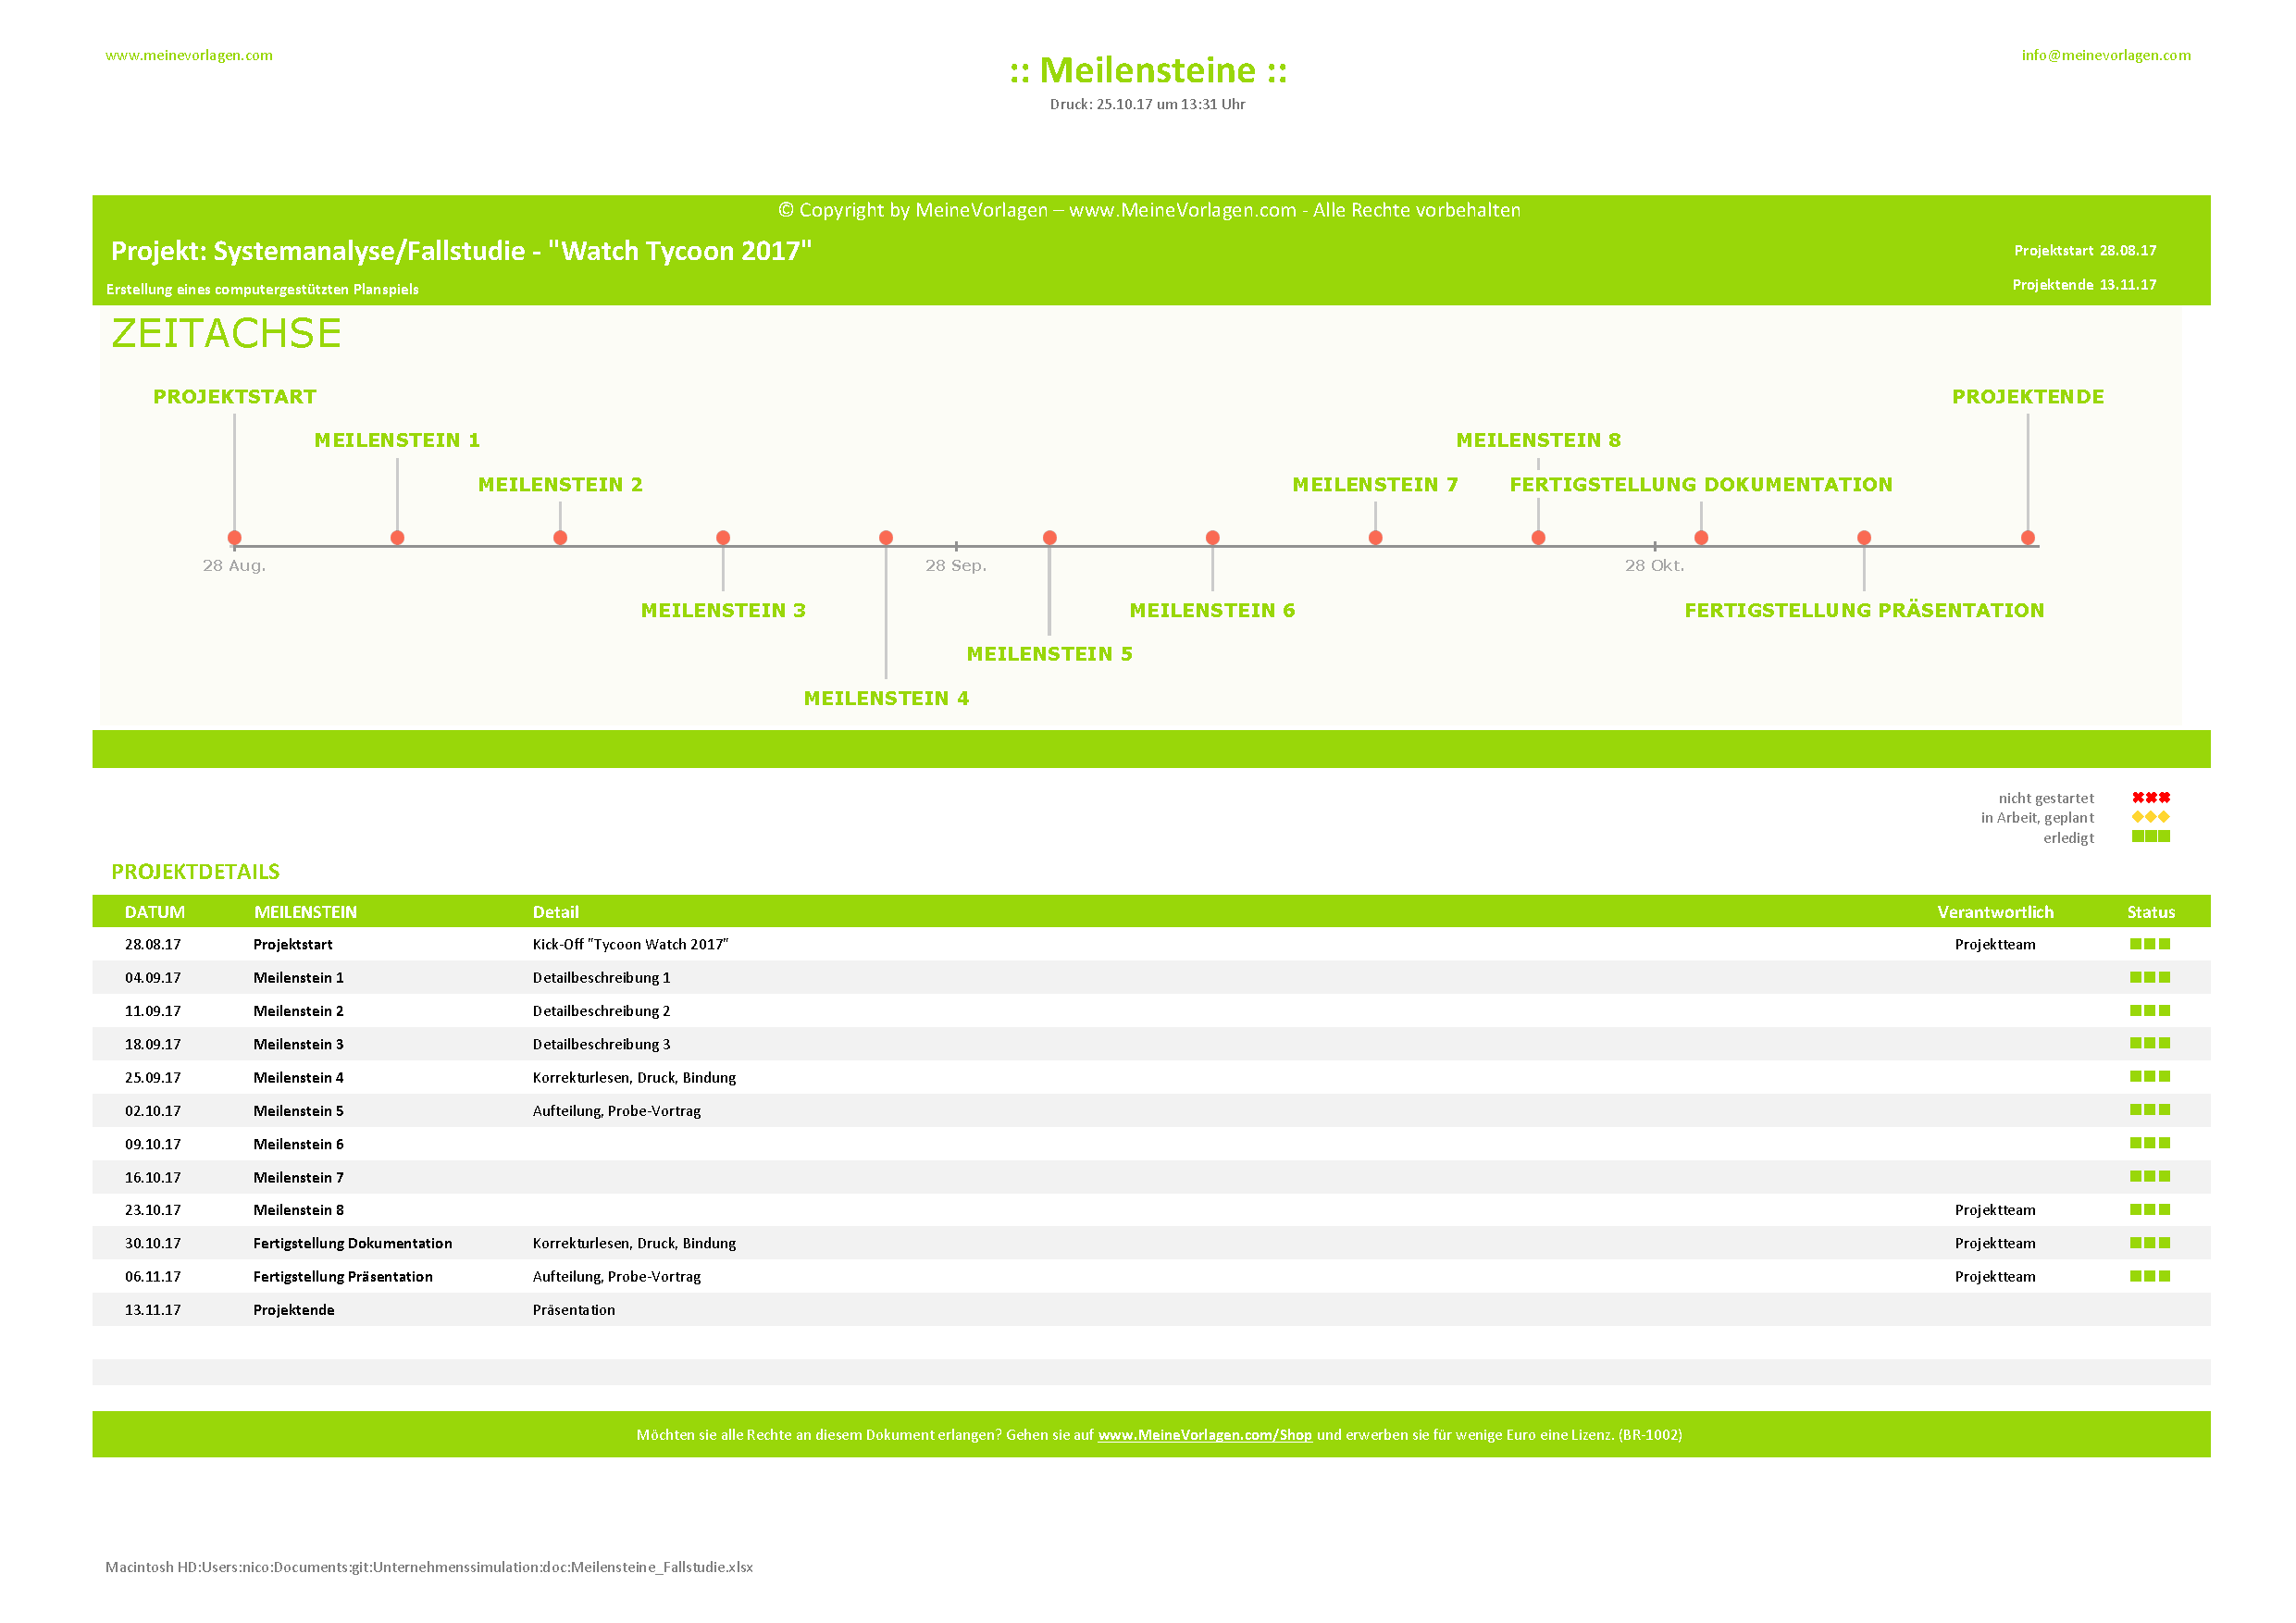
\includegraphics[angle=90, scale=0.45]{img/Meilensteine_Fallstudie.pdf}
	\label{fig:abb}
	\caption{Meilenstein-Diagramm} 
\end{figure}
